\documentclass{article}

\usepackage{amsmath,amsthm,amssymb} %Misc math symbols
\usepackage{mathtools}
\usepackage[utf8]{inputenc}
\usepackage[margin=1in]{geometry}
\usepackage{caption} 				%Inserting multiple figures
\usepackage{subcaption}
\usepackage[svgnames]{xcolor}
\usepackage{listings}
\usepackage{tikz, pgfplots} 			%Drawing pictures
\usepackage{fancyhdr} 				%Header style
\usepackage[svgnames]{xcolor}		%Coding styles
\usepackage{enumitem}				%Enumerating using letters
\usepackage{mathrsfs}				%Fonts
\usepackage{listings}

\usepackage{accents}
\newcommand{\dbtilde}[1]{\accentset{\approx}{#1}}
\newcommand{\vardbtilde}[1]{\tilde{\raisebox{0pt}[0.85\height]{$\tilde{#1}$}}}

\setlength{\headheight}{15.2pt}
\pagestyle{fancy}
\lhead{ \fancyplain{}{Andrew Kao} }
\rhead{ \fancyplain{}{Wed, Nov 13, 2019} }
\chead{ \fancyplain{}{BUS 41100: Project Proposal }}

\begin{document}

\subsection*{Research Question}

The high level research question is to look at the effect of reinforcing identity within Hispanic populations on their schooling outcomes. Specifically, I'll be using the influence of Spanish language television as the channel by which identity is reinforced, and look at how it affects everything from graduation rates to disciplinary action taken to math abilities and English proficiency for Hispanic students in public schools. In short, if I have access to more programming from my home country, does this make me less engaged in school (perhaps because there are more distractions or because it socially ostracizes me etc.), or does this make me perform better (perhaps because l have more role models or because I have something to talk with peers about in school, and hence motivation to attend/perform)?

\subsection*{Why does this matter?}

There's good reason to believe that identity, as reinforced through mass media, has a large effect on the lives people lead.   Oberholzer-Gee, Waldfogel (AER 2009) demonstrate that the presence of Spanish language local news increases Hispanic voter turnout, while Yanigazawa-Drott (QJE 2014) shows that radio broadcasts in Rwanda contributed to the violence and genocide that took place in the 90s. It would be reasonable to think then, that there could be a meaningful effect of Spanish language TV on education. 

\subsection*{Method}

To isolate the causal effect of Spanish language television, I adopt the technique used in Newman, Velez (AJPS 2019) and generalize it from three counties to the entirety of the US. Newman and Velez exploit a FCC (Federal Communications Commission) regulation which determines the distance from a TV station in which the station's broadcast signal is protected from interference. This creates a natural regression discontinuity, where the decaying strength of a signal over distance is combined with this cutoff in broadcast protection to create a split among people just inside and outside these coverage 'contours' that are presumably comparable save for their access to broadcast TV. 

In the case of Spanish language TV in particular, this should allow me to examine its causal effect on Hispanic populations for spatially located outcomes, such as public schooling results. It's worth noting that these contours are purely determined by an algorithm that looks at things like local elevation and antennae strength, so that the cutoffs are located in more or less random locations, and that coverage is large enough that these contours tend to cut across towns and suburbs, rather than cities. Finally, regressions using US census data indicate that Hispanic people do not migrate across counties in response to these contours.

A standard regression thus looks like restricting the universe of schools to only those within a small radius of the contour boundary, where the key independent variable of interest is an indicator for the school being inside or outside the boundary.

\subsection*{Data Sources}

I have already collected all (or probably all) of the data that I will need for this project.

Data for the instrument comes from both the FCC and TMS (a telecommunications company that was kind enough to let me use their API for free), and the instrument is fully constructed. The relevant data here is essentially just the coverage contour spatial data and the broadcast language of the station.

The data on public schools comes from the US government's CRDC (Civil Rights Data Collection) dataset. It's a very large dataset with a ton of outcome/control variables, but importantly, it breaks down all major variables of interest by ethnicity. These variables includes graduation rates, chronic absenteeism, suspensions, expulsions, arrests, bullying, AP test results, English proficiency, math class performances, gifted program enrolment etc., so I can look at effects on both the top and bottom end of the distribution, and examine potential mechanisms driving outcomes. These are all at the school level, and so I can run this through ArcGIS to get physical locations of these schools as well.

I get additional controls for things like population, income, density of Hispanic population etc. at the county level from IPUMS.

I don't have preliminary results yet, but am close to getting the school data in a clean enough shape where I can start running regressions.



%\begin{figure}[!hbtp]
%\centering
%\caption{The Coverage Contours of Spanish Language TV stations}
%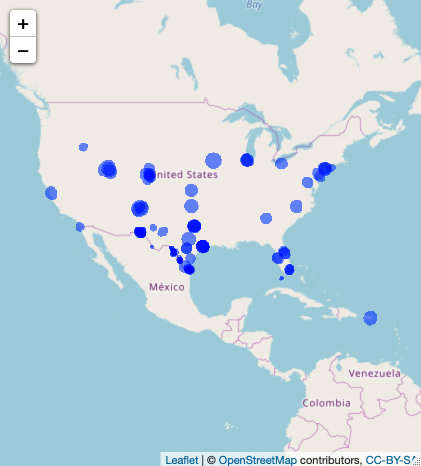
\includegraphics[width=8cm]{../analysis/Output/img/SpanishContours.png}
%\end{figure} 

%
% Table created by stargazer v.5.2.2 by Marek Hlavac, Harvard University. E-mail: hlavac at fas.harvard.edu
% Date and time: Wed, Nov 13, 2019 - 15:16:32
\begin{table}[!htbp] \centering 
  \caption{GED Completions} 
  \label{} 
\begin{tabular}{@{\extracolsep{5pt}}lccccccc} 
\\[-1.8ex]\hline 
\hline \\[-1.8ex] 
Statistic & \multicolumn{1}{c}{N} & \multicolumn{1}{c}{Mean} & \multicolumn{1}{c}{St. Dev.} & \multicolumn{1}{c}{Min} & \multicolumn{1}{c}{Pctl(25)} & \multicolumn{1}{c}{Pctl(75)} & \multicolumn{1}{c}{Max} \\ 
\hline \\[-1.8ex] 
LEA\_GEDPART\_HI\_M & 656 & 12.901 & 77.293 & 0 & 0 & 5 & 1,550 \\ 
LEA\_GEDPART\_HI\_F & 656 & 10.869 & 66.649 & 0 & 0 & 5 & 1,136 \\ 
TOT\_GEDPART\_M & 656 & 53.639 & 173.840 & 2 & 10 & 51.2 & 3,485 \\ 
TOT\_GEDPART\_F & 656 & 39.765 & 136.175 & 0 & 5 & 37 & 2,225 \\ 
LEA\_GEDCRED\_HI\_M & 656 & 2.130 & 18.292 & $-$2 & $-$2 & $-$2 & 298 \\ 
LEA\_GEDCRED\_HI\_F & 656 & 1.201 & 16.312 & $-$2 & $-$2 & $-$2 & 253 \\ 
TOT\_GEDCRED\_M & 656 & 20.870 & 55.866 & 4 & 4 & 17 & 793 \\ 
TOT\_GEDCRED\_F & 656 & 13.791 & 43.218 & $-$2 & $-$2 & 11 & 619 \\ 
\hline \\[-1.8ex] 
\end{tabular} 
\end{table} 





\end{document}
























